\begin{figure}[t]

\begin{minipage}[t]{\linewidth}

{\centering 

\begin{Shaded}
\begin{Highlighting}[]
\KeywordTok{import} \ClassTok{numpy} \KeywordTok{as} \ClassTok{np}
\KeywordTok{from} \ClassTok{poincare} \KeywordTok{import} \ClassTok{Simulator}

\VariableTok{sim} \OperatorTok{=} \ClassTok{Simulator}\KeywordTok{(\ClassTok{Oscillator})}
\VariableTok{df} \OperatorTok{=} \VariableTok{sim}.\FunctionTok{solve}\KeywordTok{(}\VariableTok{save\_at}\OperatorTok{=}\ClassTok{np}.\FunctionTok{linspace}(\ValueTok{0}, \ValueTok{5}, \ValueTok{101})\KeywordTok{)}
\end{Highlighting}
\end{Shaded}

}

\end{minipage}%
\newline
\begin{minipage}[t]{0.45\linewidth}

{\centering 

\begin{Shaded}
\begin{Highlighting}[]
\VariableTok{df}.\FunctionTok{head}\KeywordTok{()}
\end{Highlighting}
\end{Shaded}

\begin{longtable}[]{@{}lll@{}}
\toprule\noalign{}
& x & v \\
time & & \\
\midrule\noalign{}
\endhead
\bottomrule\noalign{}
\endlastfoot
0.00 & 1.000000 & 0.000000 \\
0.05 & 0.998750 & -0.049979 \\
0.10 & 0.995005 & -0.099835 \\
0.15 & 0.988772 & -0.149440 \\
0.20 & 0.980069 & -0.198672 \\
\end{longtable}

}

\end{minipage}%
\hfill
\begin{minipage}[t]{0.45\linewidth}

{\centering 

\begin{Shaded}
\begin{Highlighting}[]
\VariableTok{df}.\FunctionTok{plot}\KeywordTok{()}\OperatorTok{;}
\end{Highlighting}
\end{Shaded}

\begin{figure}[H]

{\centering 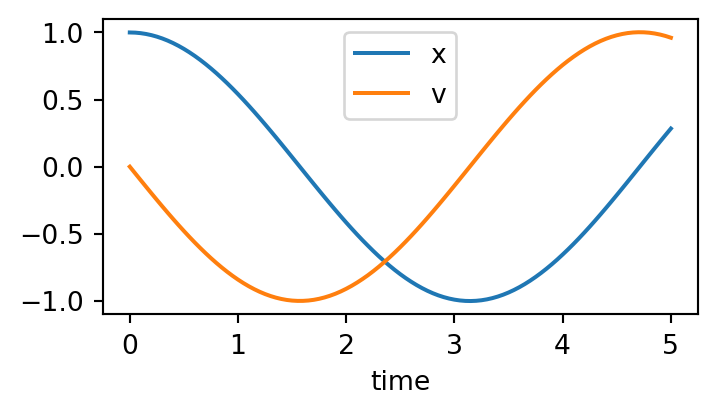
\includegraphics{article_files/figure-latex/cell-9-output-1.pdf}

}

\end{figure}

}

\end{minipage}%

\caption{\label{fig-sim}Simulation of the \texttt{Oscillator} system
from Figure~\ref{fig-second-order}. The output is a
\texttt{pandas.DataFrame} with a column for each variable and the time
as index. It is inspected and plotted with the \texttt{pandas} methods.}

\end{figure}
